% !TEX root = ../thesis_main.tex
%
%
%
%%% %%%%%%% %%%
\clearpage	
\chapter{Results and Conclusions}
\label{results_chapter}
%\section{Measured Limits on $b_{Fierz}$, $C_S$, $C_T$}
\section{Measured Limits on $b_{Fierz}$ and $\Abeta$}
\label{sec:measured_limits}

After corrections have been applied and uncertainties evaluated, statistical confidence intervals for the 2D $\Abeta$ vs $\bFierz$ parameter space are shown in Fig.~\ref{fig:2dchi2_alldata} for all datasets combined.  The final estimates of $\Abeta$ and $\bFierz$ with uncertainties at the $1\sigma$ level are given by:
\bea
\bFierz =& \,0.033  &\!\!\! \pm\, 0.084(\textrm{stat})\;\, \pm\, 0.039(\textrm{sys})  \\
\Abeta  =& -0.5738 &\!\!\! \pm\, 0.0082(\textrm{stat})    \pm\, 0.0041(\textrm{sys}), 
\eea
%
\begin{figure}[h!tb]
	\centering
	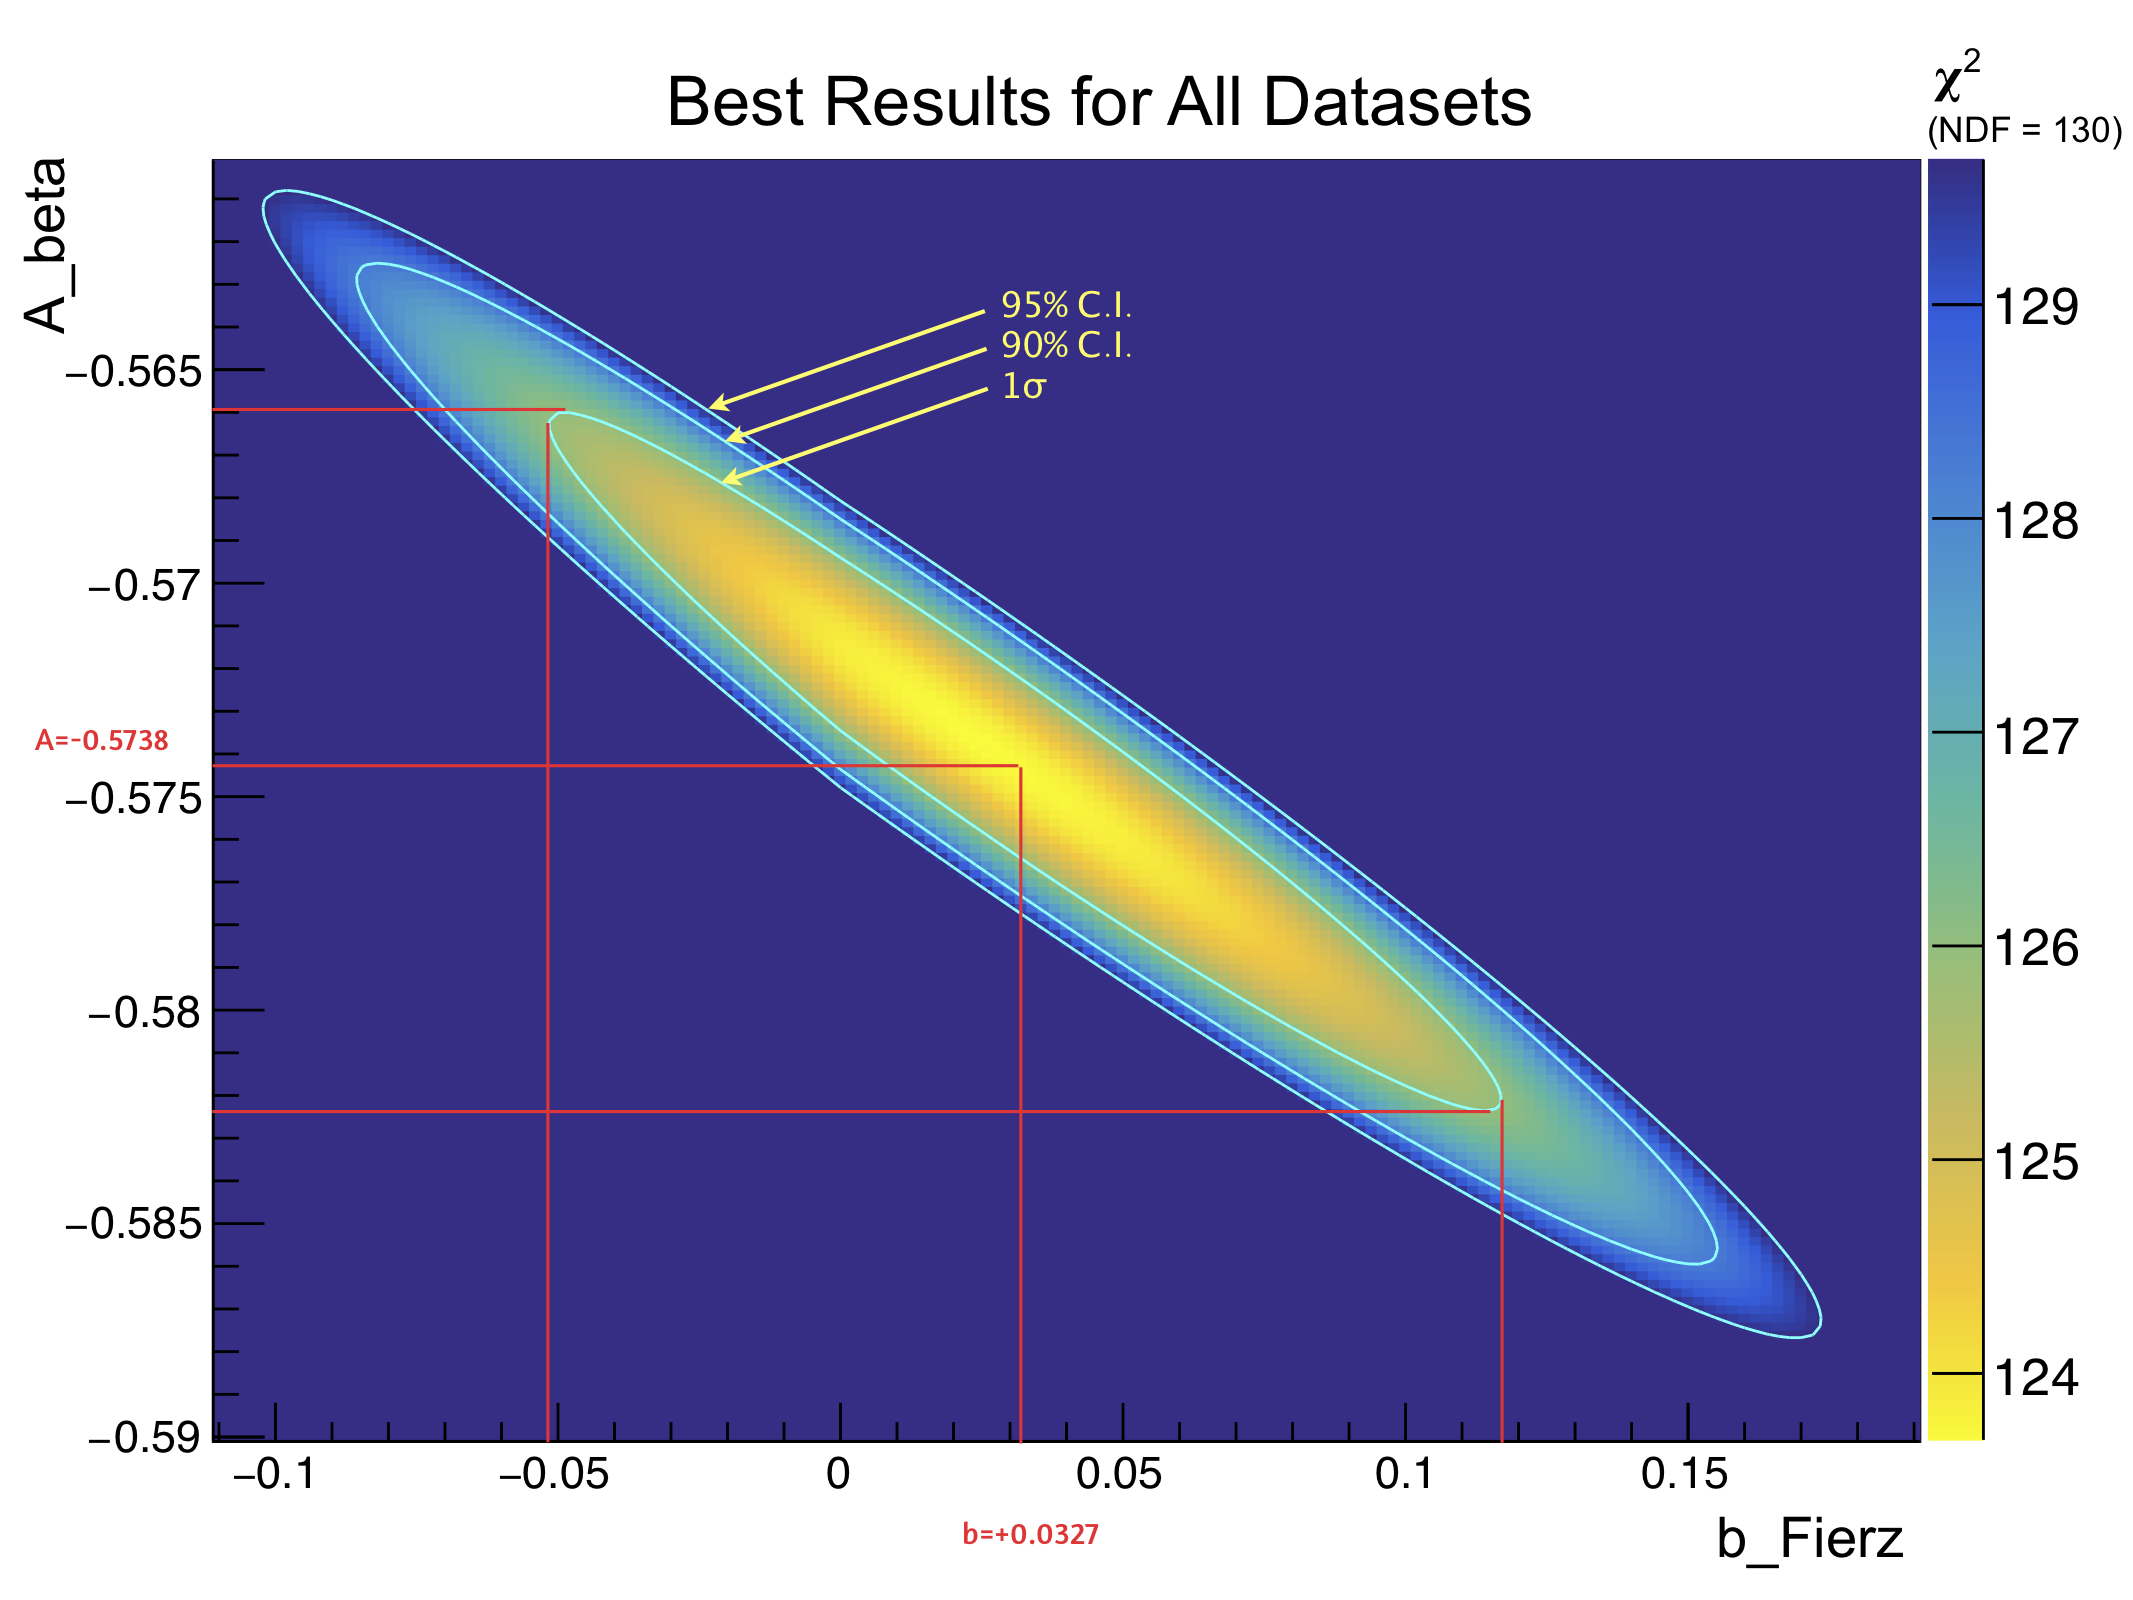
\includegraphics[width=.999\linewidth]
	{Figures/Chi2_2D_AllData.png}
	\caption[$\chi^2$ Map for All Data]{A $\chi^2$ map to compare all experimental data to a simulated parameter space of $\Abeta$ and $\bFierz$ values.  The minimum reduced $\chi^2$ value is 0.95145.  All corrections have been included, however only statistical confidence intervals are shown.  
	%\copyright~2022 Melissa Anholm.
	}	
	\label{fig:2dchi2_alldata}
\end{figure}
%
and a list of contributing uncertainties is provided in Table~\ref{table:budget}.  The error is dominated by statistics, which is unsurprising given that the superratio asymmetry has been used, thereby decreasing systematic errors in exchange for an increase in statistical errors (see Appendix~\ref{appendix:superratio} for a further discussion of the superratio and superratio asymmetry).  
% !TEX root = ../thesis_main.tex



%%%% --- * --- %%%%	
%\renewcommand{\arraystretch}{1.6}

\begin{table}[h!!!!t]
	\begin{center}
	\begin{tabular}{ l  c  c  }
		\multicolumn{1}{l}{ Source} 		& \multicolumn{2}{c}{ \;\;\; \;\;\; Uncertainty \;\;\; \;\;\; }   
		\\
		\multicolumn{1}{l}{ } 				& \multicolumn{1}{c}{\;\; $\bFierz$}   & \multicolumn{1}{c}{$\Abeta$}   	
		\\  \hline
		%%% % %%%
		Scintillator Calibration 			& 0.003								& 0.0003											
		\\
		Scintillator Threshold  			& 0.004 							& 0.0004 						
		\\
		%%% % %%%
		DSSD Individual Strip SNR 			& 0.006								& 0.0007													
		\\
		DSSD Energy Agreement	  			& 0.005 							& 0.0006 						
		\\
		DSSD Detection Radius	  			& 0.006 							& 0.0017 						
		\\
		DSSD Energy Threshold	  			& 0.005 							& 0.0005 						
		\\
		%%% % %%%
		Atomic Cloud			  			& 0.002 							& 0.0002 						
		\\
		%%% % %%%
		Background				  			& 0.004 							& 0.0003 						
		\\
		%%% % %%%
		Beta Scattering				  		& 0.031 							& 0.0025 						
		\\
		%%% % %%%
		Low Energy Tail				  		& 0.008 							& 0.0007 						
		\\
		%%% % %%%
		Mirror Thickness				  	& 0.013 							& 0.0017 						
		\\
		DSSD Thickness				 	 	& 0.013 							& 0.0017 						
		\\
		Beryllium Foil Thickness			& 0.004								& $\!\!\!\!\!\! < 0.0001$ 			
	%	\\
		%%% % %%%
		\\  \hline
		\multicolumn{1}{l}{ Total Systematics} & \multicolumn{1}{c}{0.039}  & \multicolumn{1}{c}{0.0041}
%		Total Systematics			  		& 0.056 							& 0.0055 						
		\\
		\multicolumn{1}{l}{ Statistics} 	   & \multicolumn{1}{c}{0.084}  & \multicolumn{1}{c}{0.0082}
%		Statistics				  			& 0.084 							& 0.0082 						
	%	\\  \hline
		%%% % %%%
	\end{tabular}
	\end{center}
	\caption[Error Budget]{Error budget for the two-parameter analysis for $\bFierz$ and $\Abeta$, with all data included.  All uncertainties are believed to be uncorrelated, and are added in quadrature.  Final results: 
	$\mbox{ $\bFierz = 0.033 \pm 0.084(\textrm{stat}) \pm 0.039(\textrm{sys})$ }$ and $\mbox{ $\Abeta = -0.5738 \pm 0.0082(\textrm{stat}) \pm 0.0041(\textrm{sys})$ }$. }
	\label{table:budget}
\end{table}

%\renewcommand{\arraystretch}{1}



  %\label{table:budget}

%
\note{Just write a blurb to qualitatively summarize a bunch of the stuff in Ch.~\ref{systematics_chapter}.}
%Do I want to put my error budget table here?  If not, here it is! (~\ref{table:budget}). 
\note{Other things to discuss here:  which things are dominant error sources, and how viable it would be to improve those for future experiments.}


%%%%%%% %%%%%%%%% %%%%%%%%
\section{Comparison to TRINAT's Prior $\Abeta$ Measurement}
\label{sec:compare_Abeta}
\note{Here, I have to move over some of the other section's stuff.
Also, talk about how this measurement compares with the collaboration's previous.}
The uncertainty associated with this measurement of $\Abeta$ is significantly larger than the collaboration's previous measurement of $\Abeta$ using the same data, in which the final result was $\mbox{$\Abeta = -0.5707 \pm 0.0013(\textrm{stat}) \pm 0.0013(\textrm{sys}) \pm 0.0005(\textrm{pol})$}$~\cite{ben_Abeta} before correcting for a data selection issue that only became apparent after publication.  (The third $\Abeta$ uncertainty term, labelled `pol', arises from the uncertainty in the associated nuclear polarization measurement, which is statistically independent from the other contributions and has very few systematics in common with the other terms.  This contribution is not present in the $\bFierz$ error budget because to leading order the polarization has no effect on $\bFierz$.)  In considering the collaboration's published result for $\Abeta$, it must be noted that 
the present measurement is a two-parameter measurement rather than a one-parameter measurement, so it is expected that the uncertainty associated with a single parameter should be larger.

%However, 

To evaluate whether the collaboration's previous measurement of $\Abeta$ is consistent with the results of this analysis, a thin vertical slice of Fig.~\ref{fig:2dchi2_alldata} can be extracted at $\bFierz=0$, and its projection will provide the centroid (including systematic offsets) and statistical error associated with a one-parameter analysis for $\Abeta$ --- though this method cannot produce an estimate of the extent to which systematic uncertainties might be different.  This simple check gives a one-parameter measurement of $\Abeta = -0.5714 \pm 0.0020(\textrm{stat})$.



While it is unclear why the statistical uncertainty remains so much larger in the present analysis even after eliminating one of the parameters, this one-parameter result for $\Abeta$ is at least consistent with \emph{both} the collaboration's prior uncorrected and corrected results, even after one accounts for the fact that the previous result suffered from an oversight in which some partially polarized data was not removed from the final analysis for $\Abeta$, despite the fact that this cut \emph{was} implemented in the associated polarization measurement.  This accounts for $5\%$ of the data used in that analysis, and is estimated to decrease the average polarization by approximately $0.3\%$.  
\note[tag]{Somewhere I have to say what the polarization actually was.}
An estimate of the size of the effect on the previous measurement of $\Abeta$ suggests that the true value of $\Abeta$ is likely to be $\sim 0.0016$ more negative than reported.  
%Furthermore, there is no uncertainty associated with polarization described within the present analysis, simply because to leading order there is no effect on $\bFierz$, although it strongly affects a measurement of $\Abeta$.  
Accounting for this, a more accurate one-parameter measurement might produce the result, $\mbox{$\Abeta \approx -0.5723 \pm 0.0014(\textrm{stat}) \pm 0.0013(\textrm{sys}) \pm 0.0005(\textrm{pol})$}$.



\section{Relation to Present Limits on Scalar and Tensor Interactions}
\label{sec:scalartensorlimits}
\label{sec:relation_to_other_measurements}
\note{begin literal quote from John:}
The best existing measurements of the Fierz interference term are taken from the decay of the neutron, with \mbox{$\bFierz = 0.017 \pm 0.021$} from PERKEO III being both the most precise and most recent result~\cite{Saul2020}, published only a few months after a result of $\bFierz = 0.066 \pm 0.041$(stat) $\pm 0.024$(sys) from their UCNA competitors~\cite{UCNAfierz2020}.  These results are \emph{nearly} consistent with the standard model prediction of zero at the 1-$\sigma$ level.

%consistent with the standard model prediction of zero, and with the two recent (and independent) results for the neutron's $\bFierz$ value~\cite{Saul2020,UCNAfierz2020}. 
%
Our measurement is strongly related, yet complementary.  The measured values of $\bFierz$ cannot be directly compared between the neutron and $^{37}$K, because the neutron's sensitivity to scalar and tensor couplings is different than our own.  In particular, using $\rho$ as defined in Eq.~(\ref{eq:definerho_intro})
%$\lambda := \frac{g_A M_{GT}}{g_V M_F}$, a parameter unique to a given transition (see Eq.~(\ref{eq:definelambda}) and the related discussion)
we find:
%
%In terms of non-Standard Model Lorentz current structures, to lowest order in the non-SM  currents the same equation applies:\aside{John's $\bFierz$ equation was off...}
\bea
\bFierz &=& \frac{\pm 2\gamma}{1 + \rho^2} \left( \frac{g_S}{g_V} + \rho^2 \frac{g_T}{g_A} \right)
%\bFierz = \pm \frac{(C_S +C_S') + (C_T - C_T') \lambda^2}{ 1 + \lambda^2}
\label{eq:bFierz_in_conclusion}
\eea
where the top/bottom sign is for $\beta^-$/$\beta^+$ decay, and $g_X$ ($X = \{ V,A,S,T\} $) is a purely left-handed coupling for vectors, axial-vectors, scalars, and tensors~\cite{jtw,jtw_coulomb}.
%~\aside{I think we're missing a $\gamma$.}
%(the plus is for $\beta^-$ decay and the - for $\beta^+$ decay)
In the case of $^{37}$K, a previous measurement puts $ | \rho | \approx 0.576 $, while, in the case of the neutron, the equivalent quantity within Eq.~(\ref{eq:bFierz_in_conclusion}) is 
%$| \rho | \approx 
$\sim$2.215~\cite{NeutronAbeta2018,Saul2020,UCNAfierz2020}.
\note{is it always lambda for the neutron???  ... possibly.}
%%$\lambda$ is close to $\sqrt{3/5}$ (the expected value of \mbox{$J/(J+1)$} for a single $J=3/2$, $d 3/2$ nucleon)~\cite{deShalit1963}
%%In our $^{37}$K case, $\lambda^2$ = $|M_{\rm GT}|^2$/$|M_{\rm F}|^2$ is close to 3/5 (the expected value of \mbox{$J/(J+1)$} for a single $J=3/2$, $d 3/2$ nucleon)~\cite{deShalit1963},
%%while for the neutron $\lambda^2$ is close to 3 (the expected value for a $(J+1)/J$, $J=1/2$, $s1/2$ nucleon).
The Fermi matrix element, $|M_F|$, is nearly the same for both of these isospin = 1/2 decays (the largest correction is the larger isospin mixing of $\sim$0.01 in $^{37}$K).
This means that our observable is comparatively less sensitive to Lorentz tensor currents, and will predominantly constrain or discover Lorentz scalar currents.  See Fig.~(\ref{fig:exclusionplotfromjohn}).

\note{}
\begin{figure}[h!t!b!]
	\centering
	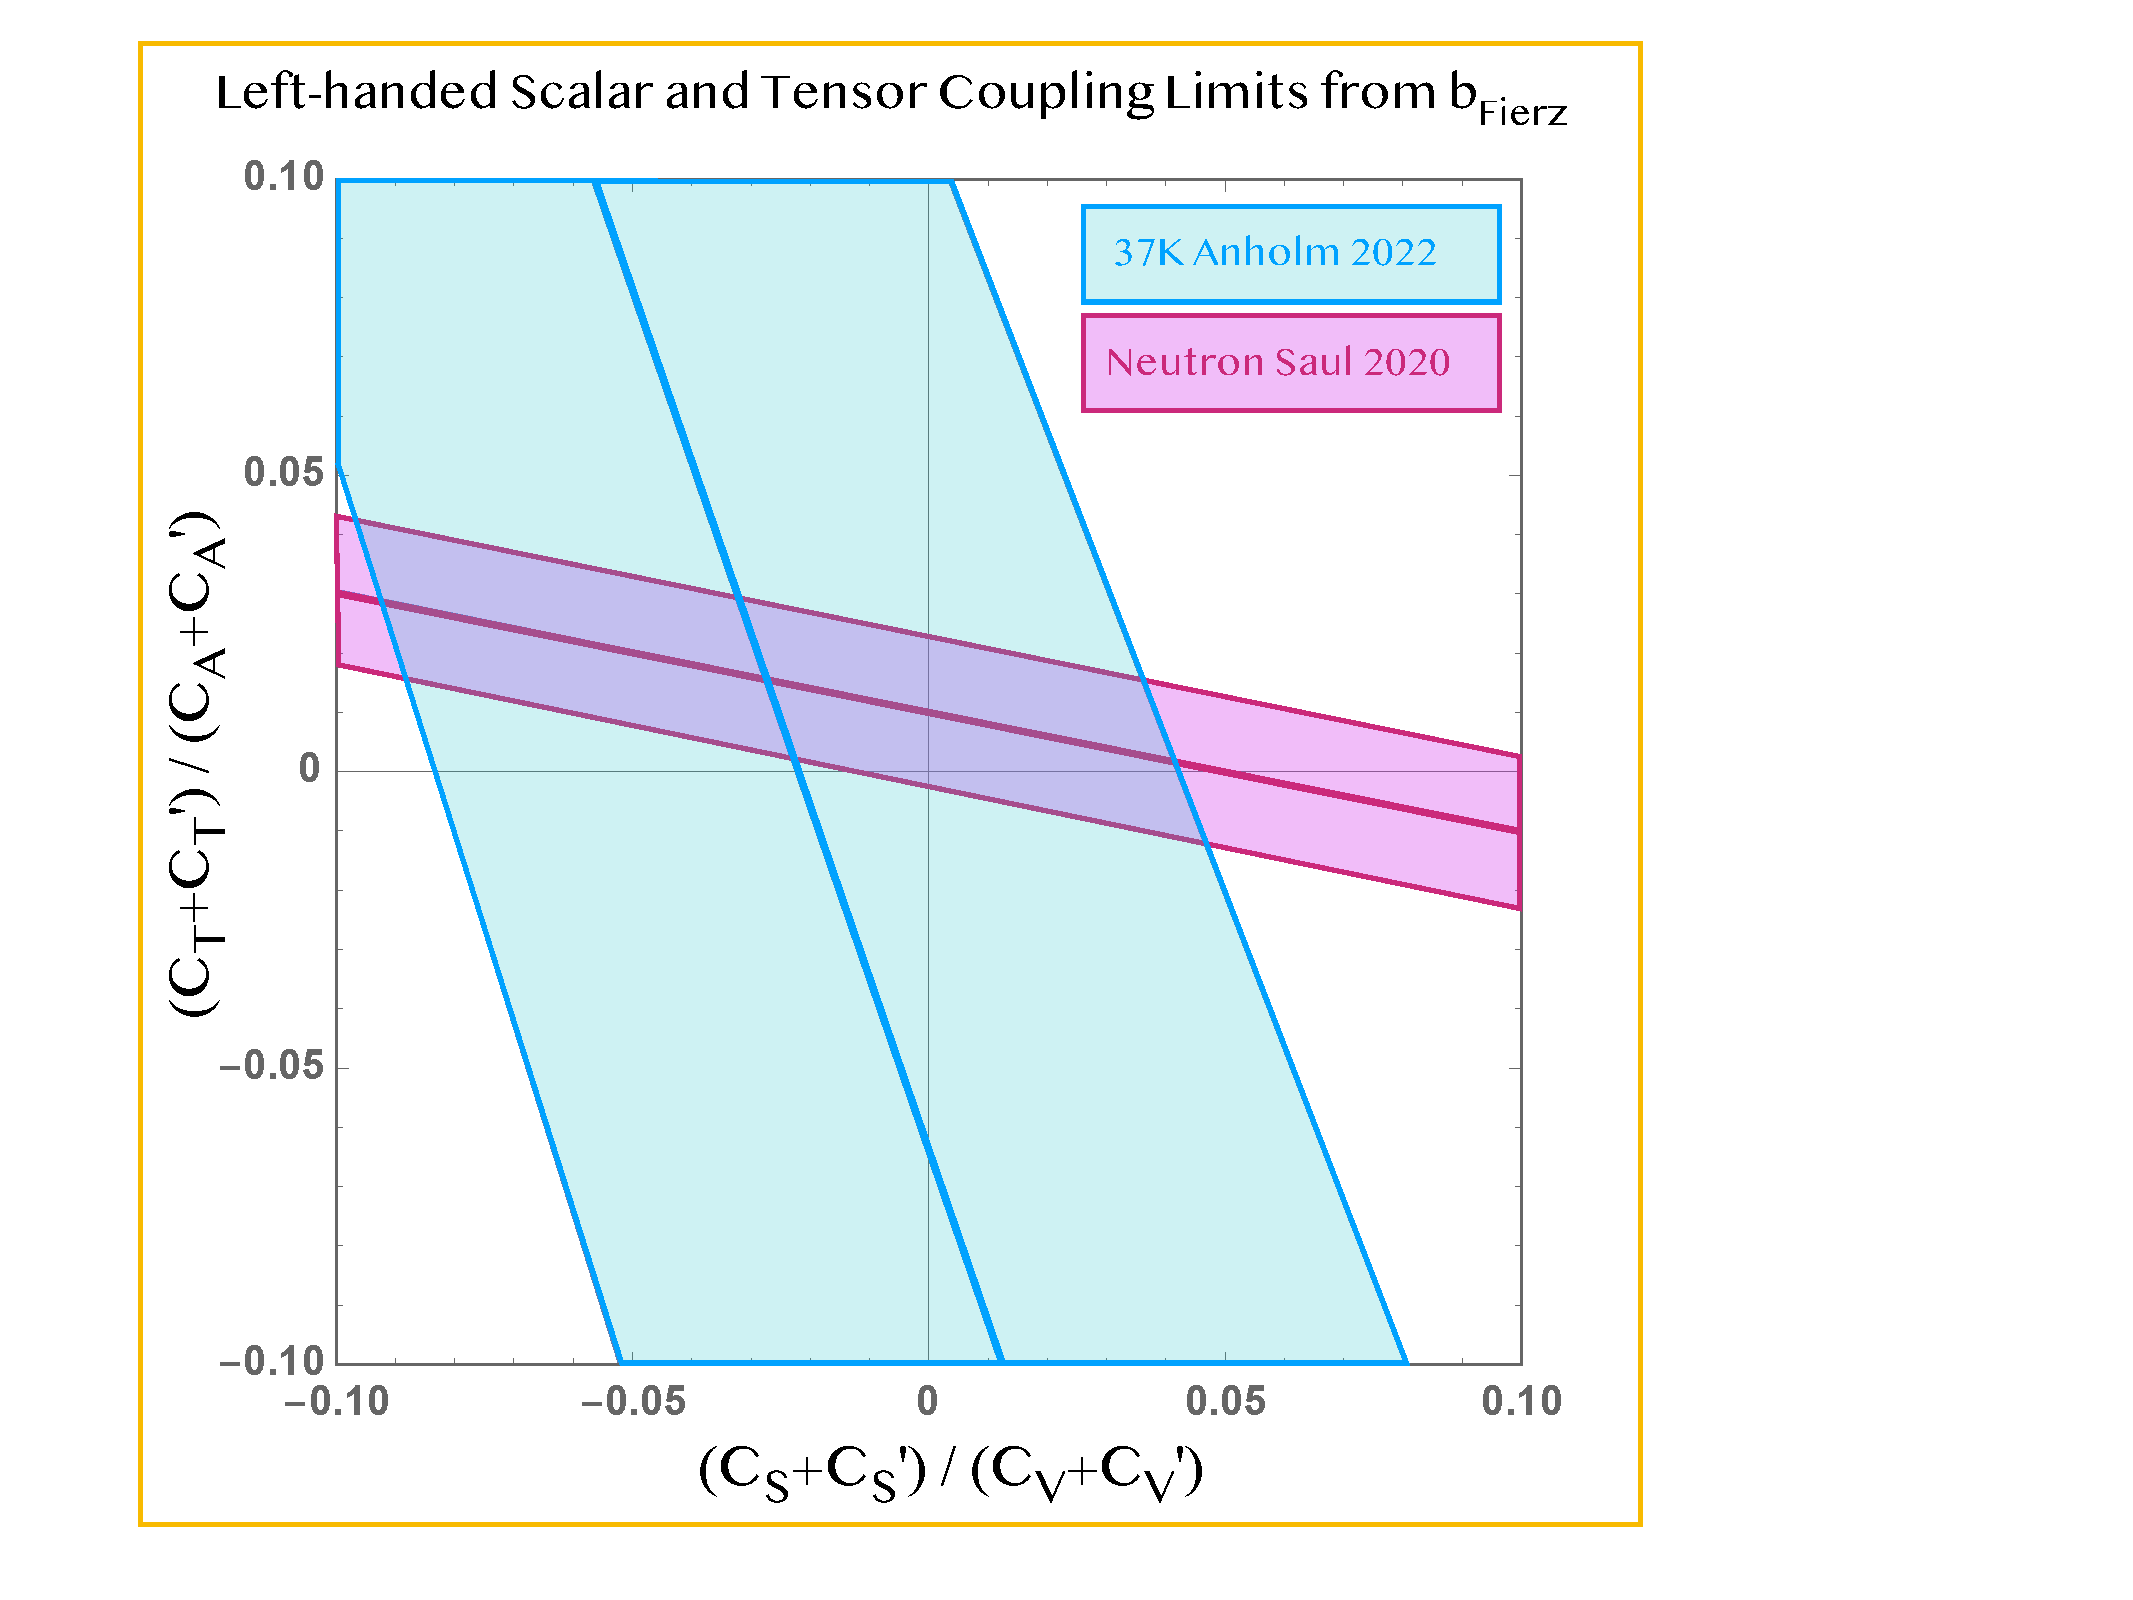
\includegraphics[width=.999\linewidth]{Figures/ScalarTensorLimits.pdf}
	\caption[An exclusion plot for left-handed scalar and tensor couplings comparing this work with the recent $\bFierz$ measurement in the neutron]{An exclusion plot comparing the measured $1\sigma$ limits for left-handed scalar and tensor couplings, comparing this work with the recent $\bFierz$ measurement in the neutron~\cite{Saul2020}.  Figure is modelled after a script provided by John Behr.  
	%\copyright~2022 Melissa Anholm.
	}
	\note{Pretty sure the sign of the $C_S$ constraint is flipped.  Also, I just can't get this centroid or these limits.  What?}
	\note[jbn]{For [bfierz exclusion plot], you have the sign correct and I don't, though I think you need $-b (1+\lambda^2)/2 = -0.02$
\\...\\
I sent the physica script.
Using your eq. 6.3, set  gs/gv = x, and gt/ga = y, rewrite the equation in y = mx + b form.
then one just substitutes the values of bf you want to plot, like maybe the centroid and the +- 1 sigma deviations from it. }
	\label{fig:exclusionplotfromjohn}
\end{figure}

However, measurements of the superallowed $0^+ \rightarrow 0^+$ beta decays are able to produce constraints on scalar couplings which are unrivaled by any other type of measurement, and improving with every experimental generation.  Though these transitions offer no sensitivity at all to tensor couplings, it would be incredibly difficult for a mixed transition measurement such as ours to compete on scalar coupling limits with the superallowed $0^+ \rightarrow 0^+$ transitions.  
At the time of writing, measurements of average $\Ebeta$ values from superallowed $0^+ \rightarrow 0^+$ transitions have together produced a constraint of \mbox{$\left| C_S / C_V \right| \leq 0.0010$} at the $1\sigma$ confidence level~\cite{HardyTownerSuperallowed2020}.

Nevertheless, it is valuable to the physics community to be able to measure observables relating to exotic physics through multiple independent experimental approaches.  As each type of measurement is necessarily sensitive to different systematic effects, the apparent redundancy of a measurement such as this one is more appropriately interpreted as a valuable cross-check. 


%At the time of writing, the superallowed $0^+ \rightarrow 0^+$ transition measurements have together produced a constraint of \mbox{$\left| C_S / C_V \right| \leq 0.0010$} at the $1\sigma$ confidence level~\cite{HardyTownerSuperallowed2020}.
\note{}

%.It would be incredibly difficult to compete with such measurements 
%
%
%in the realm of constraints to scalar couplings, 
%it is very difficult to compete with measurements from superallowed $0^+ \rightarrow 0^+$ beta decays.  Though they offer no sensitivity at all to tensor couplings, 

% offer powerful constraints .  
% Measurements of superallowed $0^+ \rightarrow 0^+$ beta decay transitions offer powerful constraints to weak force scalar couplings, but are completely unaffected by possible tensor couplings.  

%that would be very difficult to compete with by observations of a mixed transition. }

Full considerations would require a weighted fit of $\bFierz$ experiments and similar observables~\cite{Falkowski2021}, and are beyond the scope of this thesis.
The info from this thesis, values of $\Abeta$ and $\bFierz$ with their uncertainties, can together with the known $fT$ value (lifetime and
branching ratio) allow the community and/or the collaboration to include the results in a future constraint or discovery of scalar and tensor Lorentz currents
contributing to $\beta$ decay.
\note{end literal quote from John.}


%
%%%%%%% %%%%%%%%% %%%%%%%%
\FloatBarrier
\section{Possible Future Work:  $R_{\textrm{slow}}$}
\label{section_rslow}
%\subsection{Background}
As discussed in Ch.~\ref{intro_chapter}, the nuclear weak force is known to be a predominantly left-handed vector and axial-vector $(V-A)$ interaction -- meaning that immediately following an interaction (e.g. beta decay) with a weak force carrying boson ($W^+,\: W^-,\: Z$), 
normal-matter leptons (such as the electron and electron neutrino) emerge with left-handed chirality,
while the anti-leptons (e.g. the positron and electron anti-neutrino) emerge with right-handed chirality.  

In the limit of massless particles, the particle's chirality is the same as its helicity. Thus, in a left-handed model, the direction of an (ultrarelativistic) normal lepton's spin is antiparallel to its direction of motion, and the direction of spin for an anti-lepton is parallel to its direction of motion.  For a non-relativistic particle the property of chirality is fairly abstract, and describes the appropriate group representation and projection operators to be used in calculations.  It should be noted that a fully chiral model is also one which is maximally parity violating.

This odd quirk of the nuclear weak force is not only \emph{predominantly} true, but it is, to the best of our current scientific knowledge, \emph{always} true --- that is, attempts to measure any right-handed chiral components of the weak force have produced results consistent with zero~\cite{severijns_beck_cuncic_2006,severijns_cuncic_2011}.  This project proposes a further measurement to constrain the strength of the right-handed component of the weak interaction.  

Although the primary focus of this thesis is a search for exotic scalar and tensor couplings within the weak force, it is clear that a precision search for right-handed vector and axial-vector $(V+A)$ interactions would be motivated by very similar rationale.

In the proposed experiment, we focus once again on the spin-polarized decay, \mbox{$^{37}\textrm{K} \rightarrow \,^{37}\textrm{\!Ar} + \beta^{+} + \nu_e$}, exploiting the principle of conservation of angular momentum as it applies to this transition.  The proposed analysis could be performed on the data that has already been collected, although, as we will see, there are some inherent difficulties to this approach which might be eliminated with a fresh set of decay data.



%
The decay process is as described in Appendix~\ref{appendix_forthepeople}.  Within the \ac{JTW} formalism, information about the handedness of any couplings is buried within the relative signs of the primed and un-primed coupling constants ($C_X$ and $C_X^\prime$, for $X = \{ V,A,S,T\}$).  Since this section describes a search for a different type of exotic physics, it is clear that the simplifications to be made within the \ac{JTW} formalism will be different.  
% with the exception being the simplifications that can be made to the \ac{JTW} formalism.  
Recall that for the expected pure left-handed interactions, the coupling constants obey the rule, $C_X = C_X^\prime$ ($X = \{ V,A,S,T,P\}$).  For a purely right-handed interaction, the equivalent relationship is $C_X = - C_X^\prime$.  Since we know, at least for vectors and axial vectors, that the interaction must still be predominantly left-handed, one way to approach the problem is to define a new basis for the couplings to explicitly split the left-handed and right-handed couplings, as in:
\bea
C_X^{L} &:=& \frac{1}{\sqrt{2}}(C_X + C_X^\prime)
\\
C_X^{R} &:=& \frac{1}{\sqrt{2}}(C_X - C_X^\prime).
\eea

The decay may be treated as a three-body problem in which the available kinetic energy is divided up between the beta, the neutrino, and the recoiling $^{37}\textrm{\!Ar}$ nucleus, and (of course) the total linear and angular momentum are conserved.  While the neutrino cannot be detected directly, its kinematics may be reconstructed from observations of the beta and the recoiling daughter nucleus.  By placing detectors above and below the decaying atom along the axis of its polarization, we are able to obtain information about the outgoing beta's energy and momentum, in the cases of interest to us, where it is emitted along (or close to) the axis of polarization.  

It should be noted that for the class of decays of greatest interest, where the beta and the neutrino emerge back-to-back along the polarization axis, the recoiling daughter nucleus will have zero momentum along the directions perpendicular to this axis, and on average less total energy than if the beta and neutrino were emitted in a parallel direction.  Henceforth, daughter nuclei from a back-to-back decay as shown in Figure~\ref{fig:rhc} will be described as `slow' recoils.  In terms of observables, 
%these slow recoils, upon being swept into a detector by an ambient electric field, 
this means that if the electric field is configured to point along one of the axes perpendicular to the polarization direction, then when the recoiling ion is swept away into a detector, the slow recoil's hit position should be exactly along the projection of the polarization axis.  Furthermore, the slow recoil's time of flight should be in the middle of the time of flight spectrum, since other recoils will be emitted with momentum towards or away from the detector.  Of course, this is a simplistic description; in nature, no matter how strong the right-handed couplings, emitted particles will have a continuous angular spectrum -- the above is only meant to describe the angular setup which would give us maximal sensitivity to observables relating to right-handed currents.  

\begin{figure}[h!t!b!]
	\centering
	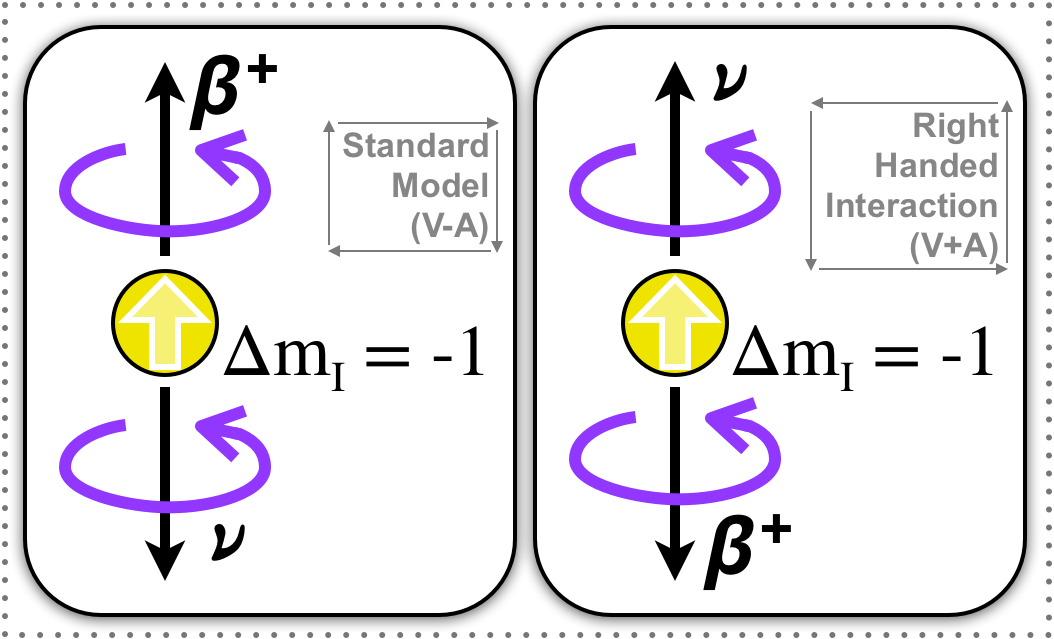
\includegraphics[width=.999\linewidth]{Figures/RHC.png}
	\caption[A Comparison of Left-Handed and Right-Handed Couplings]{A comparison of left-handed and right-handed vector and axial couplings in polarized beta decay.  The above are extremal examples;  in nature there is no requirement for the leptons to be emitted back-to-back, or for either to be emitted along the axis of polarization.  However the class of events with minimal momentum allocated to the recoiling daughter nucleus (i.e., the result of back-to-back lepton emission) is what provides the most sensitivity to the $\Rslow$ observable, and a $\beta$ coincidence (our detectors are located along the axis of polarization) is required.
	The precise scenario on the right is the only one that is \emph{completely} disallowed in the absence of right-handed couplings, and only in the relativistic limit.  For intermediate decay scenarios, the probability is simply suppressed based on the extent to which the usual left-handed coupling can access the phase space.  
	%\copyright~2022 Melissa Anholm.
	\label{fig:rhc}
	}
\end{figure}

The recoiling $^{37}\textrm{\!Ar}$ nucleus is a bit trickier to work with in some ways than an outgoing beta particle, but it is possible to do, and a necessary component of this measurement.  One useful feature of the $^{37}\textrm{K} \rightarrow \,^{37}\textrm{\!Ar}$ transition is that, in addition to the $\beta^+$ emitted in the decay itself, one or more \emph{orbital} electrons from the parent atom are typically lost.  In the majority of decay events only one orbital electron is shaken off, which results in the daughter $^{37}\textrm{\!Ar}$ atom being electrically neutral~\cite{gorelov2000,dan_thesis}.  In the remaining cases, two or more orbital electrons are lost this way, and the daughter atom is positively charged.  If we apply an electric field perpendicular to the direction of polarization, these positively charged $^{37}\textrm{\!Ar}^{(+n)}$ ions may be collected into a detector, from which hit position and time of flight information may be extracted.  The shake-off electrons are emitted with an average energy of only $\sim$ 2\,eV so to a very good approximation the other decay products are not perturbed by the presence of shake-off electrons~\cite{Levinger}.  

The potential exists to use these shake-off electrons as a tag for good events, in a way similar to what has been done in the present measurements of $\bFierz$ and $\Abeta$.  This could greatly improve the cleanliness of the spectra.  Unfortunately, within the 2014 data that has already been collected, the recoil detector and electron detector could not be made to work simultaneously.  Some of the resulting spectra are shown in Fig.~\ref{fig:RslowSpectra}.  While an analysis to search for right-handed interactions could be performed on existing data, it would likely \emph{significantly} improve the results if a new dataset were collected with both \ac{MCP} detectors working at the same time. 

\begin{figure}[htb]
	\centering
	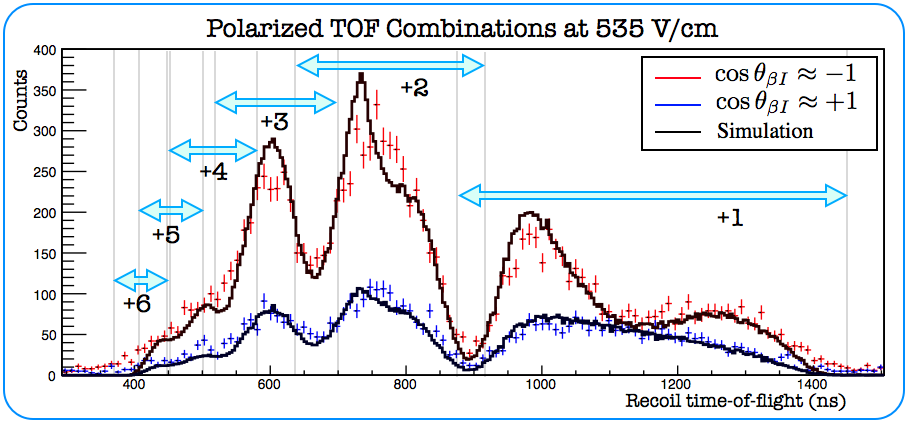
\includegraphics[width=.999\linewidth]{Figures/Rslow_tof_squished.png}
	\caption[Recoil TOF Spectra at 535 V/cm]{Recoil TOF Spectra for $^{37}$K, taken at 535 V/cm.  Recoil spectra are partially separated by charge state.  For the most part, the dips within the centre of each charge state distribution are the result of the decay chamber's geometry.  However, within these spectra, a non-zero $\Rslow$ would manifest as a change in the relative sizes of the mid-charge-state dips when comparing the red and blue spectra.	
	%\copyright~2022 Melissa Anholm.
	}
	\label{fig:RslowSpectra}
\end{figure}



In June 2014, approximately 7 days of beam time at TRIUMF was dedicated to the TRINAT $^{37}\textrm{K}$ beta decay experiment.  During this period, approximately 10,000 atoms were held within the trap at any given time.  The cleaned spectra show around 50,000 polarized beta-recoil coincidence events in total, divided among measurements at three different electric field strengths (535 V/cm, 415 V/cm, 395 V/cm).

Approximately half of this data was collected with the recoil MCP in use and is therefore suitable for use in this project to search for right-handed currents;  the other half is used as described within the rest of this document to search for scalar and tensor couplings.   

A fit to simulation has shown that the data that has already been collected has sufficient statistical power to measure the \emph{fractional} contribution of any polarized `new physics' beta decay parameter (ie right-handed, scalar, and tensor currents within the weak interaction) to a sensitivity of $\sim 2\%$ of its true value.  Systematic limitations are still being assessed.  




%%%%%% %%%%%%% %%%%%%%
\section{Summary}
This two-parameter analysis to measure $\Abeta$ and $\bFierz$ has produced the results:
\bea
\bFierz =& \,0.033  &\!\!\! \pm\, 0.084(\textrm{stat})\;\, \pm\, 0.039(\textrm{sys})  \\
\Abeta  =& -0.5738 &\!\!\! \pm\, 0.0082(\textrm{stat})    \pm\, 0.0041(\textrm{sys}),
\eea
where uncertainties are evaluated at 1$\sigma$.  This measurement of $\bFierz$ is consistent with the standard model value of $\bFierz=0$ for the absence of scalar and tensor currents, and $\Abeta$ is consistent both with the collaboration's prior measurement of $\Abeta$, as well as with the theory prediction using no exotic physics, at 
%value predicted by the standard model at
$\Abeta=-0.5706\pm0.0007$.  %\aside[tag]{somewhere, I have to define $\Abeta$ in terms of $\lambda$...} 
To date there is little credible experimental evidence for the presence of scalar or tensor interactions;  the fact that our result is consistent with $\bFierz=0$ indicates that we are in agreement with the experimental community as well.

%a non-zero $\bFierz$ value; this means that our own measured $\bFierz$ value is also consistent with the other \emph{experimental} evidence.

The result for $\bFierz$ is dominated by statistical uncertainty, suggesting that the measurement could be improved simply by counting longer.  It is unlikely, with the present apparatus, to be possible to count \emph{faster} instead, as the event rates recorded are already approaching the maximum that our data acquisition system can tolerate without causing problems.  Unfortunately, to extract $^{37}$K at a reasonable rate, a special titanium carbide target must be built and installed.  This is not a desirable target for the other research groups at TRIUMF, so they are available only infrequently.  However --- and perhaps especially in light of the present result --- it is likely that TRINAT will have access to a titanium carbide target again at some point in the future, and it will then be possible to perform an updated measurement of $\bFierz$ in $^{37}$K.

There is also room for improvement to the systematic uncertainty, which is dominated by scattering and the related measurements of material thicknesses.  
\note[tag]{Gerald says:  write another paragraph here.}
\note{begin direct quote from John:}
Largely because of this result,
the collaboration is working to reduce the largest systematics,
using lower-Z materials to reduce backscattering, and changing the silicon
$\delta$E to a multi-wire proportional chamber with very thin windows.
The collaboration has already implemented very thin pellicle mirrors.
The projected systematic uncertainty could approach 0.01 in a future
experment, which would then likely continue to be limited by statistics.
\note{end quote from John.}

%Precision measurements in nuclei are of continued interest to the scientific community as a way to search for or constrain exotic physics, and























